% Options for packages loaded elsewhere
\PassOptionsToPackage{unicode}{hyperref}
\PassOptionsToPackage{hyphens}{url}
%
\documentclass[
  11pt,
  ignorenonframetext,
]{beamer}
\usepackage{pgfpages}
\setbeamertemplate{caption}[numbered]
\setbeamertemplate{caption label separator}{: }
\setbeamercolor{caption name}{fg=normal text.fg}
\beamertemplatenavigationsymbolsempty
% Prevent slide breaks in the middle of a paragraph
\widowpenalties 1 10000
\raggedbottom
\setbeamertemplate{part page}{
  \centering
  \begin{beamercolorbox}[sep=16pt,center]{part title}
    \usebeamerfont{part title}\insertpart\par
  \end{beamercolorbox}
}
\setbeamertemplate{section page}{
  \centering
  \begin{beamercolorbox}[sep=12pt,center]{part title}
    \usebeamerfont{section title}\insertsection\par
  \end{beamercolorbox}
}
\setbeamertemplate{subsection page}{
  \centering
  \begin{beamercolorbox}[sep=8pt,center]{part title}
    \usebeamerfont{subsection title}\insertsubsection\par
  \end{beamercolorbox}
}
\AtBeginPart{
  \frame{\partpage}
}
\AtBeginSection{
  \ifbibliography
  \else
    \frame{\sectionpage}
  \fi
}
\AtBeginSubsection{
  \frame{\subsectionpage}
}

\usepackage{amsmath,amssymb}
\usepackage{iftex}
\ifPDFTeX
  \usepackage[T1]{fontenc}
  \usepackage[utf8]{inputenc}
  \usepackage{textcomp} % provide euro and other symbols
\else % if luatex or xetex
  \usepackage{unicode-math}
  \defaultfontfeatures{Scale=MatchLowercase}
  \defaultfontfeatures[\rmfamily]{Ligatures=TeX,Scale=1}
\fi
\usepackage{lmodern}
\usetheme[]{AnnArbor}
\usecolortheme{seahorse}
\ifPDFTeX\else  
    % xetex/luatex font selection
\fi
% Use upquote if available, for straight quotes in verbatim environments
\IfFileExists{upquote.sty}{\usepackage{upquote}}{}
\IfFileExists{microtype.sty}{% use microtype if available
  \usepackage[]{microtype}
  \UseMicrotypeSet[protrusion]{basicmath} % disable protrusion for tt fonts
}{}
\makeatletter
\@ifundefined{KOMAClassName}{% if non-KOMA class
  \IfFileExists{parskip.sty}{%
    \usepackage{parskip}
  }{% else
    \setlength{\parindent}{0pt}
    \setlength{\parskip}{6pt plus 2pt minus 1pt}}
}{% if KOMA class
  \KOMAoptions{parskip=half}}
\makeatother
\usepackage{xcolor}
\newif\ifbibliography
\setlength{\emergencystretch}{3em} % prevent overfull lines
\setcounter{secnumdepth}{5}


\providecommand{\tightlist}{%
  \setlength{\itemsep}{0pt}\setlength{\parskip}{0pt}}\usepackage{longtable,booktabs,array}
\usepackage{calc} % for calculating minipage widths
\usepackage{caption}
% Make caption package work with longtable
\makeatletter
\def\fnum@table{\tablename~\thetable}
\makeatother
\usepackage{graphicx}
\makeatletter
\def\maxwidth{\ifdim\Gin@nat@width>\linewidth\linewidth\else\Gin@nat@width\fi}
\def\maxheight{\ifdim\Gin@nat@height>\textheight\textheight\else\Gin@nat@height\fi}
\makeatother
% Scale images if necessary, so that they will not overflow the page
% margins by default, and it is still possible to overwrite the defaults
% using explicit options in \includegraphics[width, height, ...]{}
\setkeys{Gin}{width=\maxwidth,height=\maxheight,keepaspectratio}
% Set default figure placement to htbp
\makeatletter
\def\fps@figure{htbp}
\makeatother

\usepackage{booktabs}
\usepackage{longtable}
\usepackage{array}
\usepackage{multirow}
\usepackage{wrapfig}
\usepackage{float}
\usepackage{colortbl}
\usepackage{pdflscape}
\usepackage{tabu}
\usepackage{threeparttable}
\usepackage{threeparttablex}
\usepackage[normalem]{ulem}
\usepackage{makecell}
\usepackage{xcolor}
\usepackage{amsmath, amssymb, bbm, amstext, array, listings, mathtools, caption, color, graphics, ulem, caption, changepage, atbegshi, soul}
\hypersetup{colorlinks=true,linkcolor=red}
\usepackage{ulem}
\pdfstringdefDisableCommands{\let\sout\relax}
\makeatletter
\makeatother
\makeatletter
\makeatother
\makeatletter
\@ifpackageloaded{caption}{}{\usepackage{caption}}
\AtBeginDocument{%
\ifdefined\contentsname
  \renewcommand*\contentsname{Table of contents}
\else
  \newcommand\contentsname{Table of contents}
\fi
\ifdefined\listfigurename
  \renewcommand*\listfigurename{List of Figures}
\else
  \newcommand\listfigurename{List of Figures}
\fi
\ifdefined\listtablename
  \renewcommand*\listtablename{List of Tables}
\else
  \newcommand\listtablename{List of Tables}
\fi
\ifdefined\figurename
  \renewcommand*\figurename{Figure}
\else
  \newcommand\figurename{Figure}
\fi
\ifdefined\tablename
  \renewcommand*\tablename{Table}
\else
  \newcommand\tablename{Table}
\fi
}
\@ifpackageloaded{float}{}{\usepackage{float}}
\floatstyle{ruled}
\@ifundefined{c@chapter}{\newfloat{codelisting}{h}{lop}}{\newfloat{codelisting}{h}{lop}[chapter]}
\floatname{codelisting}{Listing}
\newcommand*\listoflistings{\listof{codelisting}{List of Listings}}
\makeatother
\makeatletter
\@ifpackageloaded{caption}{}{\usepackage{caption}}
\@ifpackageloaded{subcaption}{}{\usepackage{subcaption}}
\makeatother
\makeatletter
\@ifpackageloaded{tcolorbox}{}{\usepackage[skins,breakable]{tcolorbox}}
\makeatother
\makeatletter
\@ifundefined{shadecolor}{\definecolor{shadecolor}{rgb}{.97, .97, .97}}
\makeatother
\makeatletter
\makeatother
\makeatletter
\makeatother
\ifLuaTeX
  \usepackage{selnolig}  % disable illegal ligatures
\fi
\IfFileExists{bookmark.sty}{\usepackage{bookmark}}{\usepackage{hyperref}}
\IfFileExists{xurl.sty}{\usepackage{xurl}}{} % add URL line breaks if available
\urlstyle{same} % disable monospaced font for URLs
\hypersetup{
  pdftitle={Causality},
  pdfauthor={Macartan Humphreys},
  hidelinks,
  pdfcreator={LaTeX via pandoc}}

\title{Causality}
\author{Macartan Humphreys}
\date{}

\begin{document}
\frame{\titlepage}
\ifdefined\Shaded\renewenvironment{Shaded}{\begin{tcolorbox}[breakable, sharp corners, frame hidden, interior hidden, boxrule=0pt, borderline west={3pt}{0pt}{shadecolor}, enhanced]}{\end{tcolorbox}}\fi

\hypertarget{seccausality}{%
\section{Causality. What's a cause?}\label{seccausality}}

\hypertarget{potential-outcomes-and-the-counterfactual-approach}{%
\subsection{Potential outcomes and the counterfactual
approach}\label{potential-outcomes-and-the-counterfactual-approach}}

\begin{frame}{Potential outcomes and the counterfactual approach}
\emph{Causation as difference making}
\end{frame}

\begin{frame}{Motivation \label{po}}
\protect\hypertarget{motivation}{}
The \emph{intervention} based motivation for understanding causal
effects:

\begin{itemize}
\tightlist
\item
  We want to know if a particular intervention (like aid) caused a
  particular outcome (like reduced corruption).
\item
  We need to know:

  \begin{enumerate}
  \tightlist
  \item
    What happened?
  \item
    What would the outcome have been if there were no intervention?
  \end{enumerate}
\item
  The problem:

  \begin{enumerate}
  \tightlist
  \item
    \ldots{} this is hard
  \item
    \ldots{} this is impossible
  \end{enumerate}
\end{itemize}

The problem in 2 is that you need to know what would have happened if
things were different. You need information on a
\textbf{counterfactual}.
\end{frame}

\begin{frame}{Potential Outcomes}
\protect\hypertarget{potential-outcomes}{}
\begin{itemize}
\tightlist
\item
  For each unit, we assume that there are two \textbf{post-treatment}
  outcomes: \(Y_i(1)\) and \(Y_i(0)\).
\item
  For example, \(Y(1)\) is the outcome that \emph{would} obtain
  \emph{if} the unit received the treatment.
\item
  The \textbf{causal effect} of Treatment (relative to Control) is:
  \(\tau_i = Y_i(1) - Y_i(0)\)
\item
  Note:

  \begin{itemize}
  \tightlist
  \item
    The causal effect is defined at the \emph{individual level}.
  \item
    There is no ``data generating process'' or functional form.
  \item
    The causal effect is defined relative to something else, so a
    counterfactual must be conceivable (did Germany cause the second
    world war?).
  \item
    Are there any substantive assumptions made here so far?
  \end{itemize}
\end{itemize}
\end{frame}

\begin{frame}{Potential Outcomes}
\protect\hypertarget{potential-outcomes-1}{}
\textbf{Idea}: A causal claim is (in part) a claim about something that
did not happen. This makes it metaphysical.
\end{frame}

\begin{frame}{Potential Outcomes}
\protect\hypertarget{potential-outcomes-2}{}
Now that we have a concept of causal effects available, let's answer two
\textbf{questions}:

\begin{itemize}
\tightlist
\item
  TRANSITIVITY: If for a given unit \(A\) causes \(B\) and \(B\) causes
  \(C\), does that mean that \(A\) causes \(C\)?
\end{itemize}
\end{frame}

\begin{frame}{Potential Outcomes}
\protect\hypertarget{potential-outcomes-3}{}
Now that we have a concept of causal effects available, let's answer two
\textbf{questions}:

\begin{itemize}
\item
  TRANSITIVITY: If for a given unit \(A\) causes \(B\) and \(B\) causes
  \(C\), does that mean that \(A\) causes \(C\)?
\item
  A boulder is flying down a mountain. You duck. This saves your life.
\item
  So the boulder caused the ducking and the ducking caused you to
  survive.
\item
  So: \emph{did the boulder cause you to survive?}
\end{itemize}
\end{frame}

\begin{frame}{Potential Outcomes}
\protect\hypertarget{potential-outcomes-4}{}
CONNECTEDNESS Say \(A\) causes \(B\) --- does that mean that there is a
spatiotemporally continuous sequence of causal intermediates?
\end{frame}

\begin{frame}{Potential Outcomes}
\protect\hypertarget{potential-outcomes-5}{}
CONNECTEDNESS Say \(A\) causes \(B\) --- does that mean that there is a
spatiotemporally continuous sequence of causal intermediates?

\begin{itemize}
\tightlist
\item
  Person A is planning some action \(Y\); Person B sets out to stop
  them; person X intervenes and prevents person B from stopping person
  A. In this case Person A may complete their action, producing Y,
  without any knowledge that B and X even exist; in particular B and X
  need not be anywhere close to the action. So: \emph{did X cause Y}?
\end{itemize}
\end{frame}

\begin{frame}{Causal claims: Contribution or attribution?}
\protect\hypertarget{causal-claims-contribution-or-attribution}{}
The counterfactual model is all about contribution, not attribution,
except in a very conditional sense.

\begin{itemize}
\tightlist
\item
  Focus is on non-rival contributions
\item
  Not: what caused \(Y\) but what is the effect of \(X\)?
\item
  At most it provides a conditional account
\end{itemize}
\end{frame}

\begin{frame}{Causal claims: Contribution or attribution?}
\protect\hypertarget{causal-claims-contribution-or-attribution-1}{}
Consider an outcome \(Y\) that might depend on two causes \(X_1\) and
\(X_2\):

\[Y(0,0) = 0\] \[Y(1,0) = 0\] \[Y(0,1) = 0\] \[Y(1,1) = 1\]

What caused \(Y\)? Which cause was most important?
\end{frame}

\begin{frame}{Causal claims: Contribution or attribution?}
\protect\hypertarget{causal-claims-contribution-or-attribution-2}{}
The counterfactual model is about attribution in a very conditional
sense.

\begin{itemize}
\item
  Focus is on non-rival contributions
\item
  Not: what caused \(Y\) but what is the effect of \(X\)?
\item
  At most it provides a conditional account
\item
  This is problem for research programs that define ``explanation'' in
  terms of figuring out the things that cause \(Y\)
\item
  Real difficulties conceptualizing what it means to say one cause is
  more important than another cause. What does that mean?
\end{itemize}
\end{frame}

\begin{frame}{Causal claims: Contribution or attribution?}
\protect\hypertarget{causal-claims-contribution-or-attribution-3}{}
\emph{Erdogan's increasing authoritarianism was the most important
reason for the attempted coup}

\begin{itemize}
\tightlist
\item
  More important than Turkey's history of coups?
\item
  What does that mean?
\end{itemize}
\end{frame}

\begin{frame}{Causal claims: No causation without manipulation}
\protect\hypertarget{causal-claims-no-causation-without-manipulation}{}
\begin{itemize}
\tightlist
\item
  Some seemingly causal claims not admissible.
\item
  To get the definition off the ground, manipulation must be imaginable
  (whether practical or not)
\item
  This renders thinking about effects of race and gender difficult
\item
  What does it mean to say that Aunt Pat voted for Brexit because she is
  old?
\end{itemize}
\end{frame}

\begin{frame}{Causal claims: No causation without manipulation}
\protect\hypertarget{causal-claims-no-causation-without-manipulation-1}{}
\begin{itemize}
\tightlist
\item
  Some seemingly causal claims not admissible.
\item
  To get the definition off the ground, manipulation must be imaginable
  (whether practical or not)
\item
  This renders thinking about effects of race and gender difficult
\item
  \textbf{Compare}: What does it mean to say that Southern counties
  voted for Brexit because they have many old people?
\end{itemize}
\end{frame}

\begin{frame}{Causal claims: Causal claims are everywhere}
\protect\hypertarget{causal-claims-causal-claims-are-everywhere}{}
\begin{itemize}
\item
  Jack exploited Jill
\item
  It's Jill's fault that bucket fell
\item
  Jack is the most obstructionist member of Congress
\item
  Melania Trump stole from Michelle Obama's speech
\item
  Activists need causal claims
\end{itemize}
\end{frame}

\begin{frame}[fragile]{Causal claims: What is actually seen?}
\protect\hypertarget{causal-claims-what-is-actually-seen}{}
\begin{itemize}
\tightlist
\item
  We have talked about what's potential, now what do we \emph{observe}?
\item
  Say \(Z_i\) indicates whether the unit \(i\) is assigned to treatment
  \((Z_i=1)\) or not \((Z_i=0)\). It describes the treatment process.
  Then what we observe is: \[ Y_i = Z_iY_i(1) + (1-Z_i)Y_i(0) \]
\end{itemize}

This is sometimes called a ``switching equation''

In \texttt{DeclareDesign} \(Y\) is realised from potential outcomes and
assignment in this way using \texttt{reveal\_outcomes}
\end{frame}

\begin{frame}{Causal claims: What is actually seen?}
\protect\hypertarget{causal-claims-what-is-actually-seen-1}{}
\begin{itemize}
\item
  Say \(Z\) is a random variable, then this is a sort of data generating
  process. BUT the key thing to note is

  \begin{itemize}
  \tightlist
  \item
    \(Y_i\) is random but the randomness comes from \(Z_i\) --- the
    potential outcomes, \(Y_i(1)\), \(Y_i(0)\) are fixed
  \item
    Compare this to a regression approach in which \(Y\) is random but
    the \(X\)'s are fixed. eg:
    \[ Y \sim N(\beta X, \sigma^2) \text{ or }  Y=\alpha+\beta X+\epsilon, \epsilon\sim N(0, \sigma^2) \]
  \end{itemize}
\end{itemize}
\end{frame}

\begin{frame}{Causal claims: The estimand and the rub}
\protect\hypertarget{causal-claims-the-estimand-and-the-rub}{}
\begin{itemize}
\tightlist
\item
  The causal effect of Treatment (relative to Control) is:
  \[\tau_i = Y_i(1) - Y_i(0)\]
\item
  This is what we want to estimate.
\item
  BUT: We never can observe both \(Y_i(1)\) and \(Y_i(0)\)!
\item
  This is the \textbf{fundamental problem} (@holland1986statistics)
\end{itemize}
\end{frame}

\begin{frame}{Causal claims: The rub and the solution}
\protect\hypertarget{causal-claims-the-rub-and-the-solution}{}
\begin{itemize}
\item
  Now for some magic. We really want to estimate:
  \[ \tau_i = Y_i(1) - Y_i(0)\]
\item
  BUT: We never can observe both \(Y_i(1)\) and \(Y_i(0)\)
\item
  Say we lower our sights and try to estimate an \emph{average}
  treatment effect: \[ \tau = \mathbb{E} [Y(1)-Y(0)]\]
\item
  Now make use of the fact that
  \[\mathbb E[Y(1)-Y(0)]  = \mathbb E[Y(1)]- \mathbb E [Y(0)] \]
\item
  In words: \emph{The average of differences is equal to the difference
  of averages}; here, the average treatment effect is equal to the
  difference in average outcomes in treatment and control units.
\item
  The magic is that \emph{while we can't hope to measure the
  differences; we are good at measuring averages}.
\end{itemize}
\end{frame}

\begin{frame}{Causal claims: The rub and the solution}
\protect\hypertarget{causal-claims-the-rub-and-the-solution-1}{}
\begin{itemize}
\tightlist
\item
  So we want to estimate \(\mathbb{E} [Y(1)]\) and
  \(\mathbb{E} [Y(0)]\).
\item
  We know that we can estimate averages of a quantity by taking the
  average value from a random sample of units
\item
  To do this here we need to select a random sample of the \(Y(1)\)
  values and a random sample of the \(Y(0)\) values, in other words, we
  \textbf{randomly assign} subjects to treatment and control conditions.
\item
  When we do that we can in fact estimate:
  \[ \mathbb {E}_N[Y_i(1) | Z_i = 1) - \mathbb {E}_N(Y_i(0) | Z_i = 0]\]
  which in expectation equals:
  \[ \mathbb{E} [Y_i(1) | Z_i = 1 \text{ or } Z_i = 0] - \mathbb{E} [Y_i(0) | Z_i = 1 \text{ or } Z_i = 0]\]
\item
  This highlights a deep connection between \textbf{random assignment}
  and \textbf{random sampling}: when we do random assignment \emph{we
  are in fact randomly sampling from different possible worlds}.
\end{itemize}
\end{frame}

\begin{frame}{Causal claims: The rub and the solution}
\protect\hypertarget{causal-claims-the-rub-and-the-solution-2}{}
This provides a \textbf{positive argument} for causal inference from
randomization, rather than simply saying with randomization ``everything
else is controlled for''

\textbf{Let's discuss:}

\begin{itemize}
\tightlist
\item
  \emph{Does the fact that an estimate is unbiased mean that it is
  right?}
\item
  \emph{Can a randomization ``fail''?}
\item
  \emph{Where are the covariates?}
\end{itemize}

\textbf{Idea}: random assignment is random sampling from potential
worlds: to understand anything you find, you need to know the sampling
weights
\end{frame}

\begin{frame}{Reflection}
\protect\hypertarget{reflection}{}
\textbf{Idea}: We now have a \emph{positive} argument for claiming
unbiased estimation of the average treatment effect following random
assignment

But is the average treatment effect a quantity of \emph{social
scientific} interest?
\end{frame}

\begin{frame}{Potential outcomes: why randomization works}
\protect\hypertarget{potential-outcomes-why-randomization-works}{}
The average of the differences \(\approx\) difference of averages

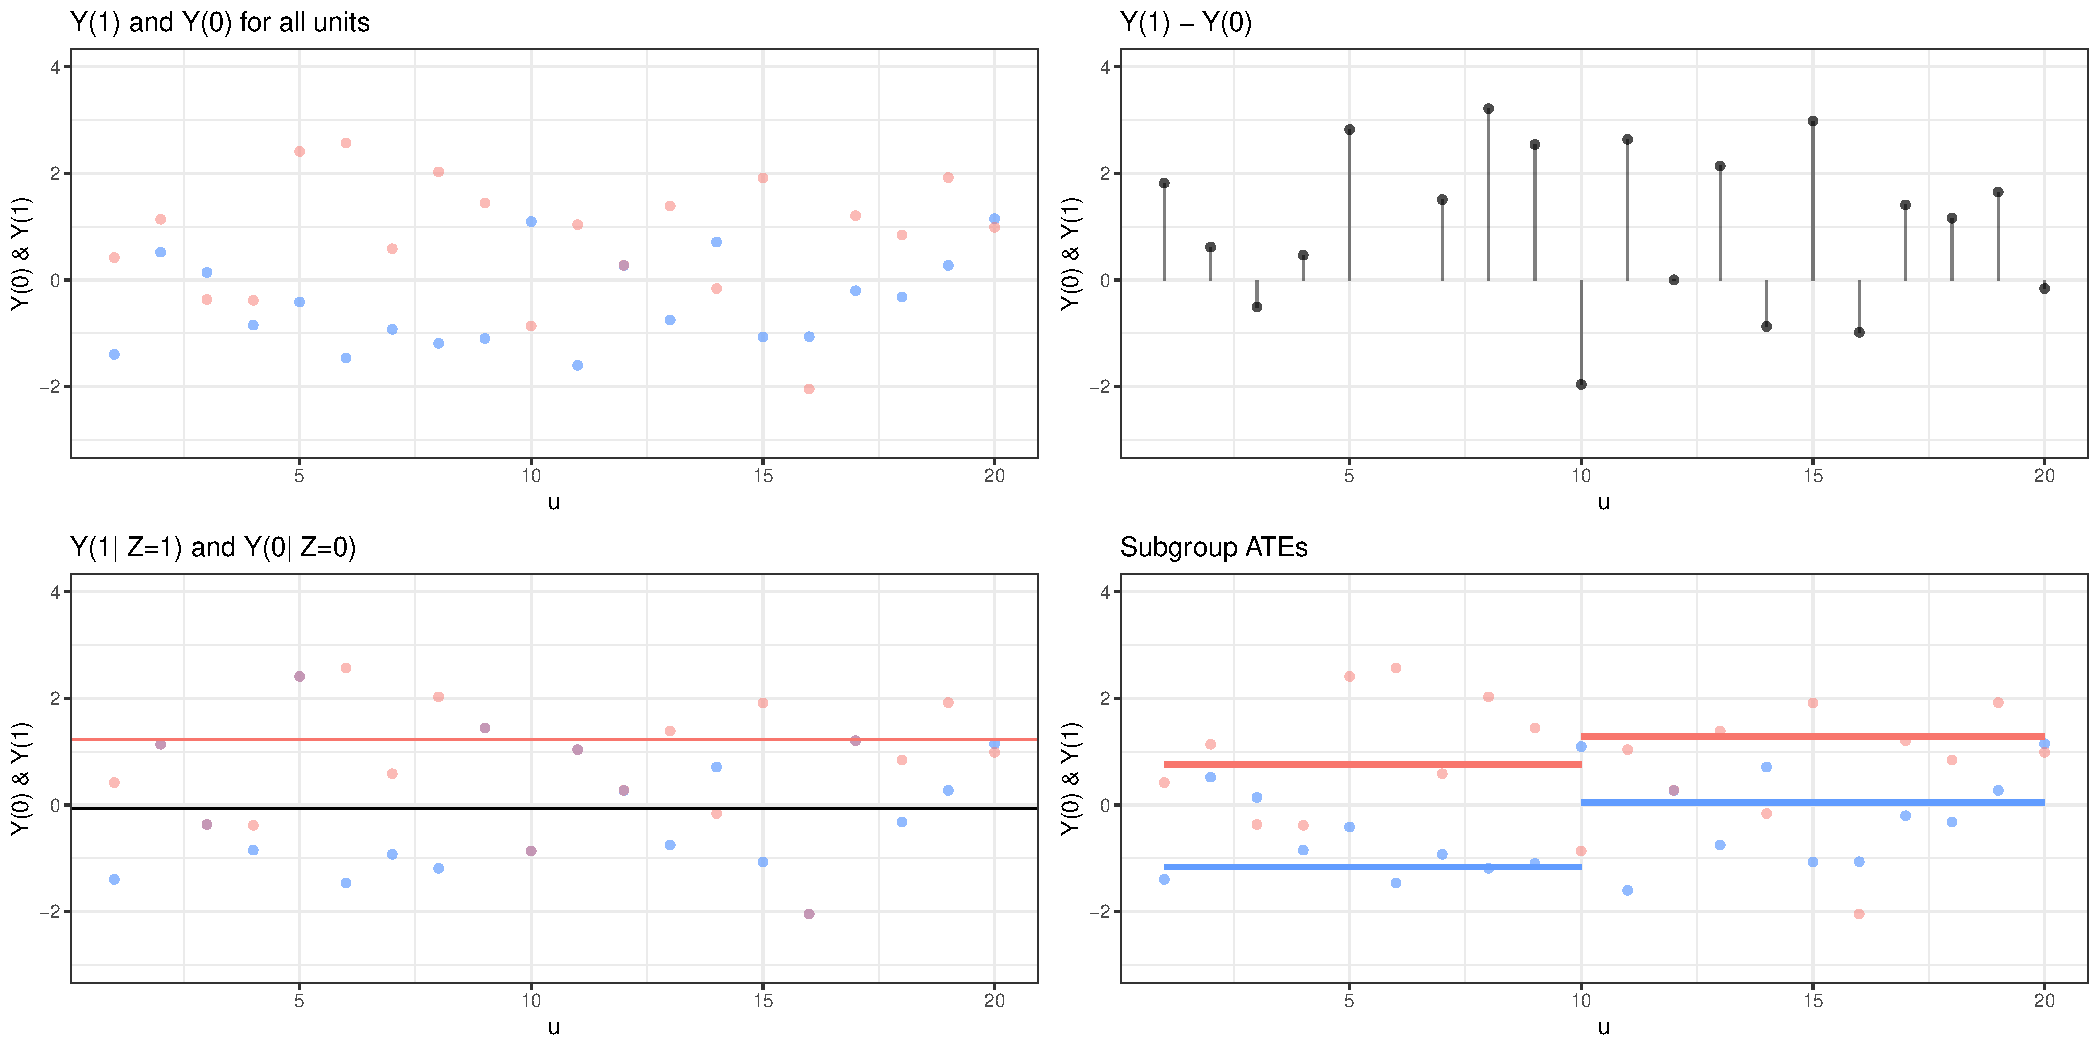
\includegraphics{2.1_causality_files/figure-beamer/unnamed-chunk-4-1.pdf}
\end{frame}

\begin{frame}{Potential outcomes: heterogeneous effects}
\protect\hypertarget{potential-outcomes-heterogeneous-effects}{}
The average of the differences \(\approx\) difference of averages

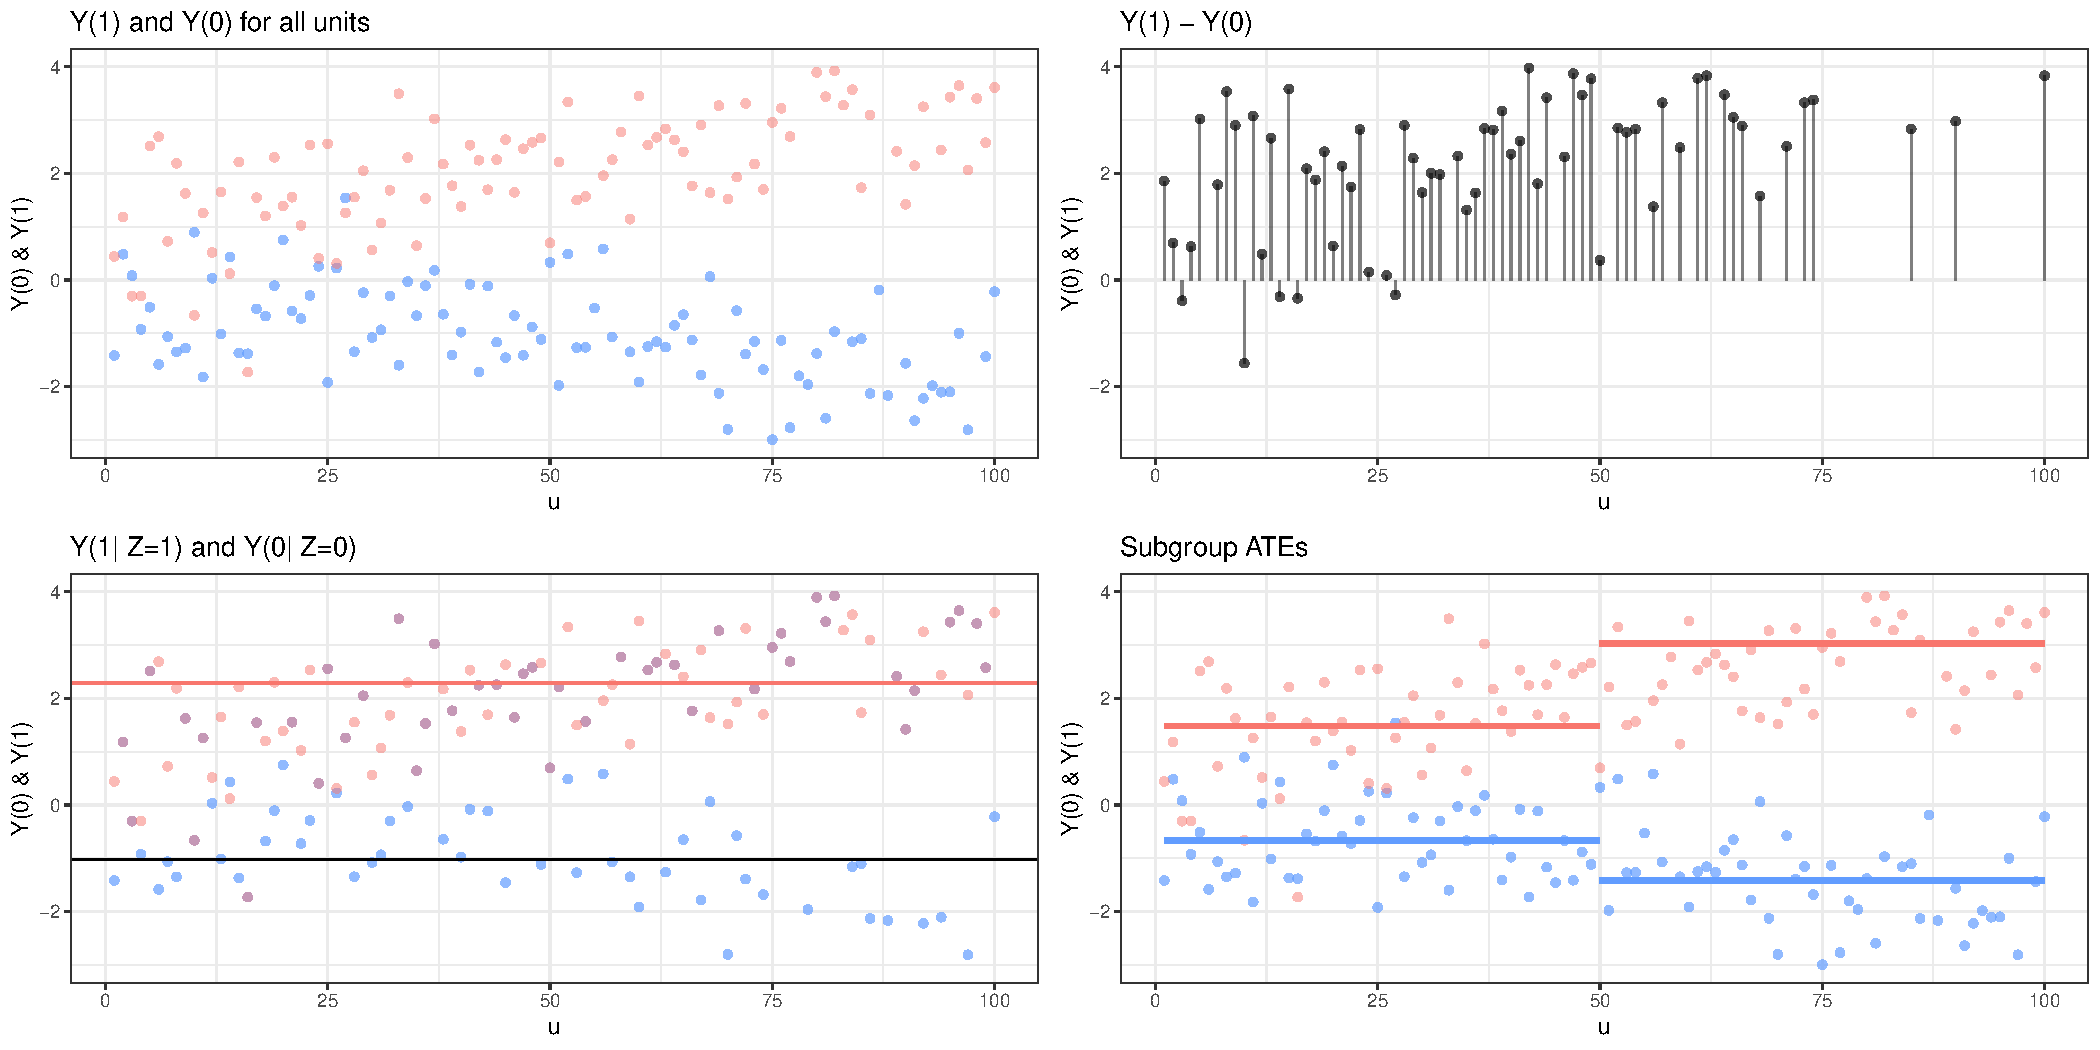
\includegraphics{2.1_causality_files/figure-beamer/unnamed-chunk-5-1.pdf}
\end{frame}

\begin{frame}{Potential outcomes: heterogeneous effects}
\protect\hypertarget{potential-outcomes-heterogeneous-effects-1}{}
\textbf{Question}: \(\approx\) or \(=\)?
\end{frame}

\begin{frame}{Exercise your potential outcomes 1}
\protect\hypertarget{exercise-your-potential-outcomes-1}{}
Consider the following potential outcomes table:

\begin{longtable}[]{@{}llll@{}}
\toprule\noalign{}
Unit & Y(0) & Y(1) & \(\tau_i\) \\
\midrule\noalign{}
\endhead
1 & 4 & 3 & \\
2 & 2 & 3 & \\
3 & 1 & 3 & \\
4 & 1 & 3 & \\
5 & 2 & 3 & \\
\bottomrule\noalign{}
\end{longtable}

\textbf{Questions for us:} What are the unit level treatment effects?
What is the average treatment effect?
\end{frame}

\begin{frame}{Exercise your potential outcomes 2}
\protect\hypertarget{exercise-your-potential-outcomes-2}{}
Consider the following potential outcomes table:

\begin{longtable}[]{@{}ccc@{}}
\toprule\noalign{}
In treatment? & Y(0) & Y(1) \\
\midrule\noalign{}
\endhead
Yes & & 2 \\
No & 3 & \\
No & 1 & \\
Yes & & 3 \\
Yes & & 3 \\
No & 2 & \\
\bottomrule\noalign{}
\end{longtable}

\textbf{Questions for us: } Fill in the blanks.

\begin{itemize}
\tightlist
\item
  Assuming a constant treatment effect of \(+1\)
\item
  Assuming a constant treatment effect of \(-1\)
\item
  Assuming an \textit{average} treatment effect of \(0\)
\end{itemize}

What is the actual treatment effect?
\end{frame}

\hypertarget{endogeneous-subgroups}{%
\subsection{\texorpdfstring{Endogeneous subgroups
\label{subs}}{Endogeneous subgroups }}\label{endogeneous-subgroups}}

\begin{frame}{Endogeneous Subgroups}
\protect\hypertarget{endogeneous-subgroups-1}{}
Experiments often give rise to endogenous subgroups. The potential
outcomes framework can make it clear why this can cause problems.
\end{frame}

\begin{frame}{Heterogeneous Effects with Endogeneous Categories}
\protect\hypertarget{heterogeneous-effects-with-endogeneous-categories}{}
\begin{itemize}
\item
  Problems arise in analyses of subgroups when the categories themselves
  are affected by treatment
\item
  Example from our work:

  \begin{itemize}
  \tightlist
  \item
    You want to know if an intervention affects reporting on violence
    against women
  \item
    You measure the share of all subjects that experienced violence that
    file reports
  \item
    The problem is that which subjects experienced violence is itself a
    function of treatment
  \end{itemize}
\end{itemize}
\end{frame}

\begin{frame}[fragile]{Heterogeneous Effects with Endogeneous
Categories}
\protect\hypertarget{heterogeneous-effects-with-endogeneous-categories-1}{}
It is possible that in truth no one's reporting behavior has changed,
what has changed is the propensity of people with different propensities
to report to experience violence:

\begin{verbatim}
\begin{table} \scriptsize
    \centering
    \begin{tabular}{rcc|cc|cc}
        
        & \multicolumn{ 2}{c}{Violence(Treatment)} & \multicolumn{ 4}{c}{Reporting(Treatment, Violence)} \\
        
        &       V(0) &       V(1) &     R(0,1) &     R(1,1) &     R(0,0) &     R(1,0) \\ \hline
        
        Type 1 (reporter) &          1 &          1 &          1 &          1 &          0 &          0 \\
        
        Type 2 (non reporter) &          1 &          0 &          0 &          0 &          0 &          0 \\          
    \end{tabular}  
\end{table}
\end{verbatim}
\end{frame}

\begin{frame}{Heterogeneous Effects with Endogeneous Categories}
\protect\hypertarget{heterogeneous-effects-with-endogeneous-categories-2}{}
\begin{itemize}
\tightlist
\item
  \textbf{Violence(Treatment)}
\item
  \textbf{Reporting(Treatment, Violence)}
\end{itemize}

\begin{longtable}[]{@{}lllllll@{}}
\toprule\noalign{}
& V(0) & V(1) & R(0,1) & R(1,1) & R(0,0) & R(1,0) \\
\midrule\noalign{}
\endhead
Type 1 (reporter) & 1 & 1 & 1 & 1 & 0 & 0 \\
Type 2 (non reporter) & 1 & 0 & 0 & 0 & 0 & 0 \\
\bottomrule\noalign{}
\end{longtable}

Expected reporting given violence in control = Pr(Type 1)

Expected reporting given violence in treatment = 100\%

\textbf{Question}: What is the actual effect of treatment on the
propensity to report violence?
\end{frame}

\begin{frame}{Heterogeneous Effects with Endogeneous Categories}
\protect\hypertarget{heterogeneous-effects-with-endogeneous-categories-3}{}
It is possible that in truth no one's reporting behavior has changed,
what has changed is the propensity of people with different propensities
to report to experience violence:

\begin{table}
\centering
\begin{tabular}{c|cc|cc|c}\scriptsize

           & \multicolumn{ 2}{c}{Reporters} & \multicolumn{ 2}{c}{Non reporters} &            \\ \hline
           & \multicolumn{ 2}{c}{Experience Violence} & \multicolumn{ 2}{c}{Experience Violence} &            \\ \hline \hline
           &         No &        Yes &        No  &        Yes &  \% Report \\

   Control &         25 &         {25} &         25 &        {25} &       { $\frac{25}{25+25}$}= 50\% \\  
   & & & & \\
  Treatment &         25 &         {25} &         50 &          {0} &      {$\frac{25}{25+0}$}=100\% \\ \hline

\end{tabular}  
\end{table}
\end{frame}

\begin{frame}{Heterogeneous Effects with Endogeneous Categories}
\protect\hypertarget{heterogeneous-effects-with-endogeneous-categories-4}{}
This problem can arise as easily in seemingly simple field experiments.
Example:

\begin{itemize}
\tightlist
\item
  In one study we provided constituents with information about
  performance of politicians
\item
  we told politicians in advance so that they could take action
\item
  we wanted to see whether voters punished poorly performing politicians
\item
  what's the problem?
\end{itemize}
\end{frame}

\begin{frame}[fragile]{Heterogeneous Effects with Endogeneous
Categories}
\protect\hypertarget{heterogeneous-effects-with-endogeneous-categories-5}{}
Question for us:

Setting:

\begin{verbatim}
    * Quotas for women are randomly placed in a set of constituencies in year 1. All winners in these areas are women; in other areas only some are. 
    * In year 2 these quotas are then lifted. 
\end{verbatim}

\textbf{Questions} Which problems face an endogenous subgroup issue?:

\begin{enumerate}
\tightlist
\item
  You want to estimate the likelihood that a woman will stand for
  reelection in treatment versus control areas in year 2.
\item
  You want to estimate how much incumbents are more likely to be
  reelected in treatment versus control areas in year 2.
\item
  You want to estimate how much treatment areas have more relected
  incumbents in elections in year 2 compared to control.
\end{enumerate}
\end{frame}

\begin{frame}{Heterogeneous Effects with Endogeneous Categories}
\protect\hypertarget{heterogeneous-effects-with-endogeneous-categories-6}{}
In such cases you can:

\begin{itemize}
\tightlist
\item
  Examine the joint distribution of multiple outcomes
\item
  Condition on pretreatment features only
\item
  Engage in mediation analysis
\end{itemize}
\end{frame}

\begin{frame}{Missing data can create an endogeneous subgroup problem}
\protect\hypertarget{missing-data-can-create-an-endogeneous-subgroup-problem}{}
\begin{itemize}
\tightlist
\item
  It is well known that missing data can undo the magic of random
  assignment.
\item
  One seemingly promising approach is to match into pairs
  \textit{ex ante} and drop pairs together \textit{ex post}.
\item
  Say potential outcomes looked like this (four units divided into two
  pairs):
\end{itemize}

\begin{longtable}[]{@{}llllll@{}}
\toprule\noalign{}
Pair & I & I & II & II & \\
\midrule\noalign{}
\endhead
Unit & 1 & 2 & 3 & 4 & Average \\
Y(0) & 0 & 0 & 0 & 0 & \\
Y(1) & -3 & 1 & 1 & 1 & \\
\(\tau\) & -3 & 1 & 1 & 1 & \\
\bottomrule\noalign{}
\end{longtable}
\end{frame}

\begin{frame}{Missing data}
\protect\hypertarget{missing-data}{}
\begin{itemize}
\item
  Say though that cases are likely to drop out of the sample if things
  go badly (eg they get a negative score or die)
\item
  Then you might see no attrition in cases in which people that are
  likely to drop out if treated do not get treated.
\item
  You might assume you have no problem (after all, no attrition).
\item
  No missing data when the normal cases happens to be selected
\end{itemize}

\begin{longtable}[]{@{}llllll@{}}
\toprule\noalign{}
Pair & I & I & II & II & \\
\midrule\noalign{}
\endhead
Unit & 1 & 2 & 3 & 4 & Average \\
Y(0) & 0 & & 0 & & 0 \\
Y(1) & & 1 & & 1 & 1 \\
\(\hat{\tau}\) & & & & & 1 \\
\bottomrule\noalign{}
\end{longtable}
\end{frame}

\begin{frame}{Missing data}
\protect\hypertarget{missing-data-1}{}
\begin{itemize}
\tightlist
\item
  But in cases in which you have attrition, dropping the pair doesn't
  necessarily help.
\item
  The problem is potential missingness still depends on potential
  outcomes
\item
  The kicker is that the method can produce bias even if (\emph{in
  fact}) there is no attrition!
\end{itemize}

Missing data when the vulnerable cases happens to be selected

\begin{longtable}[]{@{}llllll@{}}
\toprule\noalign{}
Pair & I & I & II & II & \\
\midrule\noalign{}
\endhead
Unit & 1 & 2 & 3 & 4 & Average \\
Y(0) & & {[}0{]} & 0 & & 0 \\
Y(1) & {[}-3{]} & & & 1 & 1 \\
\(\hat{\tau}\) & & & & & 1 \\
\bottomrule\noalign{}
\end{longtable}
\end{frame}

\begin{frame}{Missing data}
\protect\hypertarget{missing-data-2}{}
Note: The right way to think about this is that bias is a property of
the strategy over possible realizations of data and not normally a
property of the estimator conditional on the data.
\end{frame}

\begin{frame}{Multistage games}
\protect\hypertarget{multistage-games}{}
Multistage games can also present an endogenous group problem since
collections of late stage players facing a given choice have been
created by early stage players.
\end{frame}

\begin{frame}{Multistage games}
\protect\hypertarget{multistage-games-1}{}
Question: Does \textbf{visibility} alter the extent to which subjects
follow norms to punish antisocial behavior (and reward prosocial
behavior)? Consider a trust game in which we are interested in how
information on receivers affects their actions

\begin{table}[h!] \scriptsize
  \centering
  \caption{Return rates given investments under different conditions}
    \begin{tabular}{lp{3.8cm}|c|cc}
          &                                         & \% invested   & \multicolumn{2}{c}{Average \% returned}  \\ \hline 
          &                                         & (average)     & ...when       & ...when \\ 
          &                                         &               & 10\% invested     & 50\% invested \\ \hline \hline 
Treatment & Masked information on respondents       & 30\% (avg)    & 20\%          & 40\% \\
          & Full information on respondents         & 30\% (avg)    & 0\%           & 60\% \\
    \end{tabular}
\end{table}

What do we think? Does visibility make people react more to investments?
\end{frame}

\begin{frame}{Multistage games}
\protect\hypertarget{multistage-games-2}{}
Imagine you could see all the potential outcomes, and they looked like
this:

\begin{table}[h!] \scriptsize
  \centering
  \caption{Potential outcomes with (and without) identity protection}
    \begin{tabular}{ll|cccccc|c} \footnotesize
          &       & \multicolumn{6}{c}{Responder's return decision (given type)}& Avg.  \\ \hline 
          &       & Nice  & Nice  & Nice  & Mean  & Mean  & Mean \\ 
          & & 1&2&3&4&4&6\\ \hline \hline 
    Offerer  & Invest 10\%: & 60\%      &  60\%     &  60\%     & 0\%   & 0\%   & 0\% & 30\%\\
    behavior      & Invest 50\%: & 60\% & 60\% & 60\% &    0\%   &    0\%   &  0\% & 30\%\\
    \end{tabular}%
\end{table}

\textbf{Conclusion}: Both the offer and the information condition are
\textbf{completely irrelevant} for all subjects.
\end{frame}

\begin{frame}{Multistage games}
\protect\hypertarget{multistage-games-3}{}
Unfortunately you only see a sample of the potential outcomes, and that
looks like this:

\begin{table}[h!] \scriptsize
  \centering
  \caption{Outcomes when respondent \textbf{is visible}}
    \begin{tabular}{ll|cccccc|c} \footnotesize
          &       & \multicolumn{6}{c}{Responder's return decision (given type)}& Avg.   \\ \hline
          &       & Nice  & Nice  & Nice  & Mean  & Mean  & Mean  \\ 
                    & & 1&2&3&4&4&6\\ \hline \hline  
    Offerer  & Invest 10\%: &       &       &       & 0\%   & 0\%   & 0\% & 0\%\\
    behavior      & Invest 50\%: & 60\% & 60\% & 60\% &       &    &   &  60\% \\
    \end{tabular}
\end{table}

\textbf{False Conclusion}: When not protected, responders condition
behavior \textit{strongly} on offers (because offerers can select on
type accurately)
\end{frame}

\begin{frame}{Multistage games}
\protect\hypertarget{multistage-games-4}{}
Unfortunately you only see a sample of the potential outcomes, and that
looks like this:

\begin{table}[h!] \scriptsize
  \centering
  \caption{Outcomes when respondent \textbf{is not visible}}
    \begin{tabular}{ll|cccccc|c} \footnotesize
          &       & \multicolumn{6}{c}{Responder's return decision (given type)} & Avg.  \\ \hline
          &       & Nice  & Nice  & Nice  & Mean  & Mean  & Mean  \\ 
                    & & 1&2&3&4&4&6\\ \hline \hline  
    Offerer         & Invest 10\%: &        &       &    60\%   &    & 0\%   &      0\% & 20\%\\
    behavior        & Invest 50\%: & 60\%   &  60\% &           & 0\%      &       &   &  40\%\\
    \end{tabular}
\end{table}

\textbf{False Conclusion}: When protected, responders condition behavior
less strongly on offers (because offerers can select on type less
accurately)
\end{frame}

\begin{frame}{Multistage games}
\protect\hypertarget{multistage-games-5}{}
What to do?

\textbf{Solutions?}

\begin{enumerate}
\tightlist
\item
  Analysis \emph{could} focus on the effect of treatment on respondent
  behavior, directly.

  \begin{itemize}
  \tightlist
  \item
    This would get the correct answer but to a different question
    {[}Does information affect the share of contributions returned by
    subjects on average? No{]}
  \end{itemize}
\item
  \textbf{Strategy method} can sometimes help address the problem,
  \textbf{but} that is also (a) changing the question and (b) putting
  demands on respondent imagination and honesty
\item
  First mover action could be \textbf{directly manipulated}, but unless
  deception is used that is also changing the question
\item
  First movers could be \textbf{selected} because they act in
  predictable ways (bordering on deception?)
\end{enumerate}

\textbf{Idea}: Proceed with extreme caution when estimating effects
beyond the first stage.
\end{frame}

\hypertarget{dags}{%
\subsection{DAGs}\label{dags}}

\hypertarget{key-insight}{%
\subsection{Key insight}\label{key-insight}}

\begin{frame}{Key insight}
The most powerful results from the study of DAGs are procedures for
figuring out when conditioning aids or hinders causal identification.

\begin{itemize}
\tightlist
\item
  You can read off a \textbf{confounding} variable from a DAG.

  \begin{itemize}
  \tightlist
  \item
    You have to condition on such a variable for causal identification.
  \end{itemize}
\item
  You can read off \textbf{``colliders''} from a DAG

  \begin{itemize}
  \tightlist
  \item
    Sometimes you have \emph{avoid} conditioning on these
  \end{itemize}
\item
  Sometimes a variable might be both, so

  \begin{itemize}
  \tightlist
  \item
    you have to condition on it
  \item
    you have to avoid conditioning on it
  \item
    Ouch.
  \end{itemize}
\end{itemize}
\end{frame}

\hypertarget{key-resource}{%
\subsection{Key resource}\label{key-resource}}

\begin{frame}{Key resource}
\begin{itemize}
\item
  Pearl's book \emph{Causality} is the key reference.
  @pearl2009causality (Though see also older work such as
  @pearl1985graphoids)
\item
  There is a lot of excellent material on Pearl's page
  http://bayes.cs.ucla.edu/WHY/
\item
  See also excellent material on Felix Elwert's page
  http://www.ssc.wisc.edu/\textasciitilde felwert/causality/?page\_id=66
\end{itemize}
\end{frame}

\hypertarget{challenge-for-us}{%
\subsection{Challenge for us}\label{challenge-for-us}}

\begin{frame}{Challenge for us}
\begin{itemize}
\item
  Say you don't like graphs. Fine.\\
\item
  Consider this causal structure:

  \begin{itemize}
  \tightlist
  \item
    \(Z = f_1(U_1, U_2)\)
  \item
    \(X = f_2(U_2)\)
  \item
    \(Y = f_3(X, U_1)\)
  \end{itemize}
\end{itemize}

Say \(Z\) is temporally prior to \(X\); it is correlated with \(Y\)
(because of \(U_1\)) and with \(X\) (because of \(U_2\)).

\textbf{Question:} Would it be useful to ``control'' for \(Z\) when
trying to estimate the effect of \(X\) on \(Y\)?
\end{frame}

\hypertarget{challenge-for-us-1}{%
\subsection{Challenge for us}\label{challenge-for-us-1}}

\begin{frame}{Challenge for us}
\begin{itemize}
\item
  Say you don't like graphs. Fine.\\
\item
  Consider this causal structure:

  \begin{itemize}
  \tightlist
  \item
    \(Z = f_1(U_1, U_2)\)
  \item
    \(X = f_2(U_2)\)
  \item
    \(Y = f_3(X, U_1)\)
  \end{itemize}
\end{itemize}

\textbf{Question:} Would it be useful to ``control'' for \(Z\) when
trying to estimate the effect of \(X\) on \(Y\)?

\textbf{Answer:} Hopefully by the end of today you should see that that
the answer is obviously (or at least, plausibly) ``no.''
\end{frame}

\hypertarget{conditional-independence}{%
\subsection{Conditional independence}\label{conditional-independence}}

\begin{frame}{Conditional independence}
Variable sets \(A\) and \(B\) are conditionally independent, given \(C\)
if for all \(a\), \(b\), \(c\):

\[\Pr(A = a | C = c) = \Pr(A = a | B = b, C = c)\]

Informally; given \(C\), knowing \(B\) tells you nothing more about
\(A\).
\end{frame}

\hypertarget{causal-graphs-basics-1}{%
\subsection{Causal graphs basics 1}\label{causal-graphs-basics-1}}

\begin{frame}{Causal graphs basics 1}
\begin{itemize}
\tightlist
\item
  Consider a situation with variables \(X_1, X_2, \dots X_n\)
\item
  The probability of outcome \(x\) can always be written in the form
  \(P(X_1 = x_1)P(X_2 = x_2|X_1=x_1)(X_3 = x_3|X_1=x_1, X_2 = x_2)\dots\).
\item
  This can be done with any ordering of variables.
\item
  However the representation can be greatly simplified if you can make
  use of a set of ``parentage'' relationships
\item
  Given an ordering of variables, the \textbf{Markovian parents} of
  variable \(X_j\) are the minimal set of variables such that when you
  condition on these, \(X_j\) is independent of all other prior
  variables in the ordering
\item
  In this case we can write: \(P(x) = \prod_j(x_j | pa_j)\)
\item
  No graphs yet
\end{itemize}
\end{frame}

\hypertarget{causal-graphs-basics-2}{%
\subsection{Causal graphs basics 2}\label{causal-graphs-basics-2}}

\begin{frame}{Causal graphs basics 2}
\begin{itemize}
\tightlist
\item
  We want to use causal graphs to represent these relations of
  conditional independence.
\item
  Informally, an arrow, \(A \rightarrow B\) means that \(A\) is a cause
  of \(B\): that is, under some conditions, a change in \(A\) produces a
  change in \(B\).

  \begin{itemize}
  \tightlist
  \item
    Arrows carry no information about the type of effect; e.g.~sign,
    size, or whether different causes are complements or substitutes
  \end{itemize}
\item
  We say that arrows point from \emph{parents} to \emph{children}, and
  by extension from \emph{ancestors} to \emph{descendants}.
\item
  These are parents \emph{on the graph}; but we will connect them to
  Markovian parents in a probability distribution \(P\).
\end{itemize}
\end{frame}

\hypertarget{causal-graphs-basics-2-1}{%
\subsection{Causal graphs basics 2}\label{causal-graphs-basics-2-1}}

\begin{frame}{Causal graphs basics 2}
\begin{itemize}
\tightlist
\item
  A DAG is just a graph in which some or all nodes are connected by
  \emph{directed} edges (arrows) and there are no cyclical paths along
  these directed edges.
\item
  Consider a DAG, \(G\), and consider the ancestry relations implied by
  \(G\): the distribution \(P\) is \emph{Markov relative to the graph
  \(G\)} if every variable is independent of its nondescendants (in
  \(G\)) conditional on its parents (in \(G\)).

  \begin{itemize}
  \tightlist
  \item
    This is the \textbf{Markov condition}: conditional on its parents, a
    variable is independent of its non-descendants.
  \end{itemize}
\item
  OK now we have a link from probability distributions to graphs. But we
  have not talked about causality.
\end{itemize}
\end{frame}

\hypertarget{causal-graphs-basics-3}{%
\subsection{Causal graphs basics 3}\label{causal-graphs-basics-3}}

\begin{frame}[fragile]{Causal graphs basics 3}
We want the graphs to be able to represent the effects of interventions.

Pearl uses \texttt{do} notation to capture this idea.

\[\Pr(X_1, X_2,\dots | do(X_j = x_j))\] or

\[\Pr(X_1, X_2,\dots | \hat{x}_j)\]

denotes the distribution of \(X\) when a particular node (or set of
nodes) is intervened upon and forced to a particular level, \(x_j\).
\end{frame}

\hypertarget{causal-graphs-basics-3-1}{%
\subsection{Causal graphs basics 3}\label{causal-graphs-basics-3-1}}

\begin{frame}{Causal graphs basics 3}
Note, in general:
\[\Pr(X_1, X_2,\dots | do(X_j = x_j')) \neq \Pr(X_1, X_2,\dots | X_j = x_j')\]
as an example we might imagine a situation where for men binary \(X\)
always causes \(Y=1\) and for women \(Y=1\) regardless of \(X\). We
imagine that \(X=1\) for men only.

In that case \(\Pr(Y=1 | X = 1) = 1\) but \(\Pr(Y=1 | do(X = 1)) = .5\)
\end{frame}

\hypertarget{causal-graphs-basics-3-2}{%
\subsection{Causal graphs basics 3}\label{causal-graphs-basics-3-2}}

\begin{frame}[fragile]{Causal graphs basics 3}
\begin{itemize}
\item
  Let \(P_{z}\) denote the resulting distribution on all variables that
  arises when vector \(Z\) is ``set'' (forced, controlled\dots) to the
  value \(z\). That is when we have \texttt{do(Z=z)}.
\item
  Let \(P_*\) denote the set of all such distributions that can result
  from any set of interventions on variables.
\item
  A DAG, \(G\), is a \textbf{causal Bayesian network compatible with
  \(P_*\)} iff, for all interventions \(z\):

  \begin{enumerate}
  \tightlist
  \item
    \(P_{z}\) is Markov relative to \(G\)
  \item
    \(P_z(x_i)=1\) for all \(x_i\) consistent with \(z\)
  \item
    \(P_z(x_j|pa_j)=P(x_j|pa_j)\) for all \(x_j \not\in Z\) when
    \(pa_j\) is consistent with \(z\)
  \end{enumerate}
\end{itemize}
\end{frame}

\hypertarget{causal-graphs-basics-3-3}{%
\subsection{Causal graphs basics 3}\label{causal-graphs-basics-3-3}}

\begin{frame}[fragile]{Causal graphs basics 3}
\begin{itemize}
\tightlist
\item
  That all means that the probability distribution resulting from
  setting some set \(X_i\) to \(\hat{x'}_i\)
  (i.e.~\texttt{do(X=x\textquotesingle{})}) is:
\end{itemize}

\[P_{\hat{x}_i}=P(x_1,x_2,\dots x_n|\hat{x}_i) = \prod_{-i}P(x_j|pa_j)\mathbb{1}(x_i = x_i')\]

This means that there is only probability mass on vectors in which
\(x_i = x_i'\) (reflecting the success of control) and all other
variables are determined by their parents, given the values that have
been set for \(x_i\).
\end{frame}

\hypertarget{conditional-independence-and-d-separation}{%
\subsection{\texorpdfstring{Conditional Independence and
\(d\)-separation}{Conditional Independence and d-separation}}\label{conditional-independence-and-d-separation}}

\begin{frame}{Conditional Independence and \(d\)-separation}
\begin{itemize}
\item
  We now have a well defined sense in which the arrows on a graph
  represent a causal structure and capture the conditional independence
  relations implied by the causal structure.
\item
  Of course any graph might represent many different probability
  distributions \(P\)
\item
  We can now start reading off from a graph when there is or is not
  conditional independence between sets of variables
\end{itemize}
\end{frame}

\hypertarget{conditional-independence-on-paths}{%
\subsection{Conditional independence on
paths}\label{conditional-independence-on-paths}}

\begin{frame}{Conditional independence on paths}
\begin{figure}

{\centering 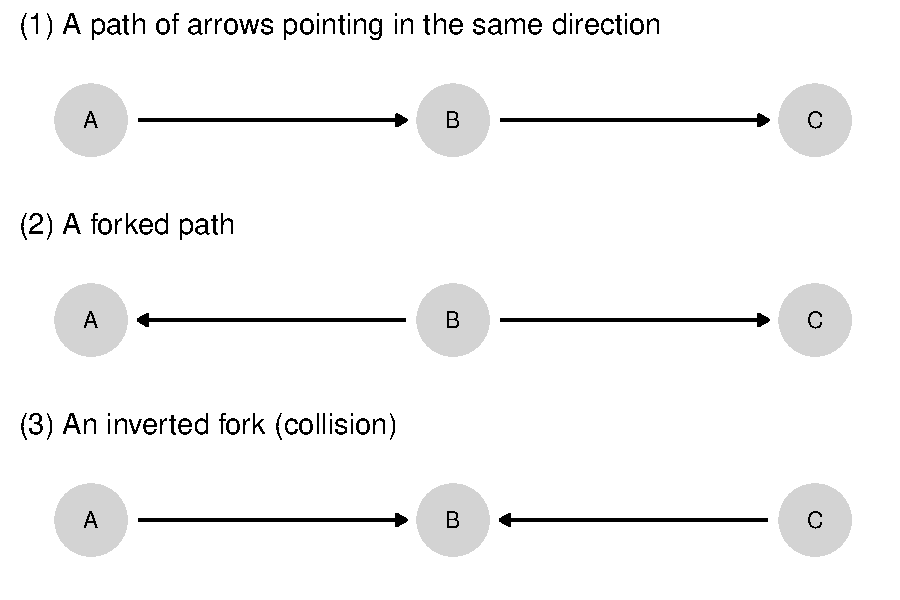
\includegraphics[width=0.7\textwidth,height=\textheight]{2.1_causality_files/figure-beamer/HJ-F-2-4-1.pdf}

}

\caption{Three elemental relations of conditional independence.}

\end{figure}
\end{frame}

\hypertarget{conditional-independence-1}{%
\subsection{Conditional independence}\label{conditional-independence-1}}

\begin{frame}{Conditional independence}
\(A\) and \(B\) are \emph{conditionally independent}, given \(C\) if on
\emph{every} path between \(A\) and \(B\):

\begin{itemize}
\tightlist
\item
  there is some chain (\(\bullet\rightarrow \bullet\rightarrow\bullet\)
  or \(\bullet\leftarrow \bullet\leftarrow\bullet\)) or fork
  (\(\bullet\leftarrow \bullet\rightarrow\bullet\)) with the central
  element in \(C\),
\end{itemize}

or

\begin{itemize}
\tightlist
\item
  there is an inverted fork
  (\(\bullet\rightarrow \bullet\leftarrow\bullet\)) with the central
  element (and its descendants) \emph{not} in \(C\)
\end{itemize}

Notes:

\begin{itemize}
\tightlist
\item
  In this case we say that \(A\) and \(B\) are d-separated by \(C\).
\item
  \(A\), \(B\), and \(C\) can all be sets
\item
  Note that a path can involve arrows pointing any direction
  \(\bullet\rightarrow \bullet\rightarrow \bullet\leftarrow \bullet\rightarrow\bullet\)
\end{itemize}
\end{frame}

\hypertarget{test-yourself}{%
\subsection{Test yourself}\label{test-yourself}}

\begin{frame}{Test yourself}
\begin{figure}

{\centering 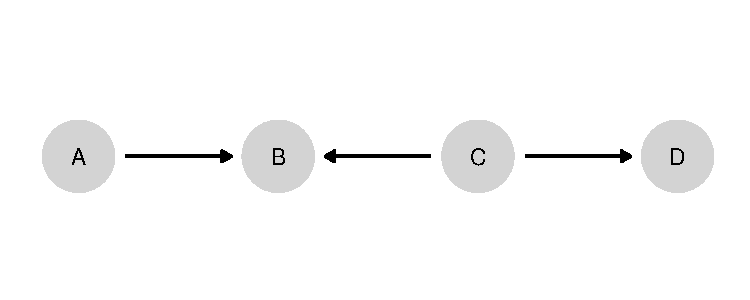
\includegraphics{2.1_causality_files/figure-beamer/unnamed-chunk-7-1.pdf}

}

\end{figure}

Are A and D unconditionally independent:

\begin{itemize}
\tightlist
\item
  if you do not condition on anything?
\item
  if you condition on B?
\item
  if you condition on C?
\item
  if you condition on B and C?
\end{itemize}
\end{frame}

\hypertarget{back-to-this-example}{%
\subsection{Back to this example}\label{back-to-this-example}}

\begin{frame}[fragile]{Back to this example}
\begin{verbatim}
* $Z = f_1(U_1, U_2)$
* $X = f_2(U_2)$
* $Y = f_3(X, U_1)$
\end{verbatim}

\begin{enumerate}
\tightlist
\item
  Let's graph this
\item
  Now: say we removed the arrow from \(X\) to \(Y\)

  \begin{itemize}
  \tightlist
  \item
    Would you expect to see a correlation between \(X\) and \(Y\) if you
    did not control for \(Z\)
  \item
    Would you expect to see a correlation between \(X\) and \(Y\) if you
    did control for \(Z\)
  \end{itemize}
\end{enumerate}
\end{frame}

\hypertarget{from-graphs-to-causal-models}{%
\subsection{From graphs to Causal
Models}\label{from-graphs-to-causal-models}}

\begin{frame}{From graphs to Causal Models}
A ``\textbf{causal model}'' is:

1.1: An ordered list of \(n\) endogenous nodes,
\(\mathcal{V}= (V^1, V^2,\dots, V^n)\), with a specification of a range
for each of them

1.2: A list of \(n\) exogenous nodes,
\(\Theta = (\theta^1, \theta^2,\dots , \theta^n)\)

2: A list of \(n\) functions \(\mathcal{F}= (f^1, f^2,\dots, f^n)\), one
for each element of \(\mathcal{V}\) such that each \(f^i\) takes as
arguments \(\theta^i\) as well as elements of \(\mathcal{V}\) that are
\emph{prior} to \(V^i\) in the ordering

and

3: A probability distribution over \(\Theta\)
\end{frame}

\hypertarget{from-graphs-to-causal-models-1}{%
\subsection{From graphs to Causal
Models}\label{from-graphs-to-causal-models-1}}

\begin{frame}{From graphs to Causal Models}
\begin{figure}

{\centering 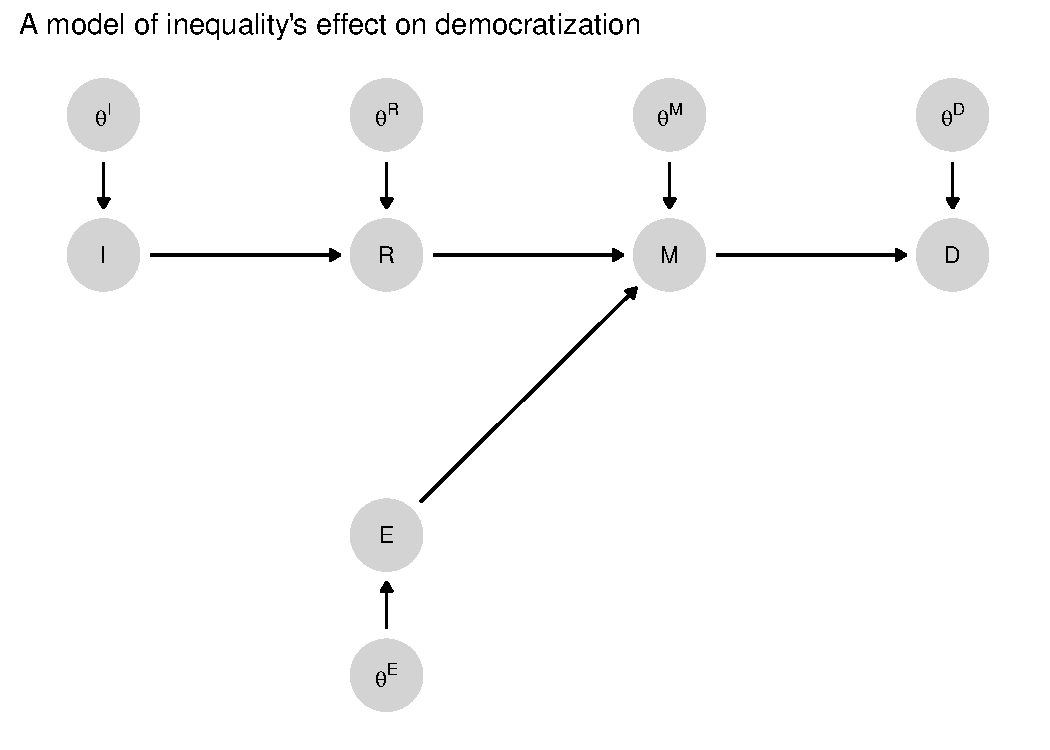
\includegraphics[width=0.8\textwidth,height=\textheight]{2.1_causality_files/figure-beamer/HJ-F-2-1-1.pdf}

}

\caption{A simple causal model in which high inequality (\(I\)) affects
democratization (\(D\)) via redistributive demands (\(R\)) and mass
mobilization (\(M\)), which is also a function of ethnic homogeneity
(\(E\)). Arrows show relations of causal dependence between variables.}

\end{figure}
\end{frame}

\begin{frame}{Effects on a DAG}
\protect\hypertarget{effects-on-a-dag}{}
Learning about effects \emph{given} a model means learning about \(F\)
and \emph{also} the distribution of shocks (\(\Theta\)).

For discrete data this can be reduced to a question about learning about
the distribution of \(\Theta\) only.
\end{frame}

\hypertarget{recap-key-features-of-graphs}{%
\subsection{Recap: Key features of
graphs}\label{recap-key-features-of-graphs}}

\begin{frame}{Recap: Key features of graphs}
\begin{itemize}
\tightlist
\item
  Directed
\item
  Acyclic
\item
  The missing arcs are the really important ones
\item
  Implicitly there are shocks going into every node
\item
  These graphs represent Nonparametric structural equation models NPSEMs
\item
  But you cannot read off the size or direction of effects from a DAG
\end{itemize}
\end{frame}

\begin{frame}{Recap: Ten things you need to know about causal inference}
\protect\hypertarget{recap-ten-things-you-need-to-know-about-causal-inference}{}
\begin{enumerate}
\tightlist
\item
  A causal claim is a statement about what didn't happen.
\item
  There is a fundamental problem of causal inference.
\item
  You can estimate average causal effects even if you cannot observe any
  individual causal effects.
\item
  If you know that \(A\) causes \(B\) and that \(B\) causes \(C\), this
  does not mean that you know that \(A\) causes \(C\).
\item
  The counterfactual model is primarily about contribution, and about
  attribution in a limited sense.
\item
  \(X\) can cause \(Y\) even if there is no ``causal path'' connecting
  \(X\) and \(Y\).
\item
  Correlation is not causation.
\item
  \(X\) can cause \(Y\) even if \(X\) is not a necessary condition or a
  sufficient condition for \(Y\).
\item
  Estimating average causal effects does not require that treatment and
  control groups are identical.
\item
  There is no causation without manipulation.
\end{enumerate}

\url{http://egap.org/resources/guides/causality/}
\end{frame}



\end{document}
